In einem Lift hängen die Kabine (mit Fahrgästen \mKO) und ein Gegengewicht (\mGO) an den beiden Enden eines Seils über eine Rolle oben im Schacht. Angenommen, der Motor fällt aus, die Rolle dreht sich frei, und die Fangbremsen greifen noch nicht. Reibung und die Massen von Seil und Rolle sind vernachlässigbar. Rechne mit \gO.

\begin{center}
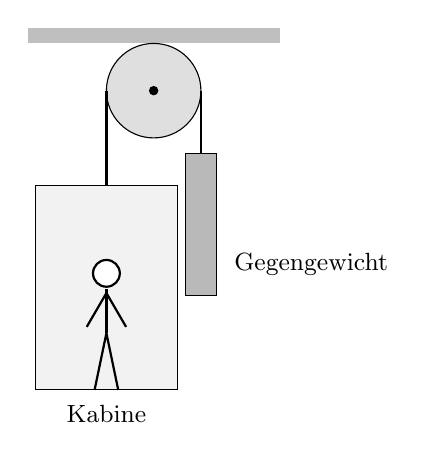
\begin{tikzpicture}[>=stealth]
 \fill[gray!50] (-1.6,3.4) rectangle (1.6,3.6);
 \draw[thick] (0,3.4) -- (0,2.8);
 \draw[fill=gray!25] (0,2.8) circle (0.6);
 \fill (0,2.8) circle (0.06);
 \draw[thick] (-0.6,2.8) -- (-0.6,1.6) (0.6,2.8) -- (0.6,2.0);
 \draw[fill=gray!10] (-1.5,-1.0) rectangle (0.3,1.6);
 \draw[thick] (-0.75,-1) -- (-0.6,-0.28) -- (-0.45,-1);
 \draw[thick] (-0.6,-0.28) -- (-0.6,0.28);
 \draw[thick, fill=white] (-0.6,0.48) circle (0.17);
 \draw[thick] (-0.6,0.23) -- (-0.85,-0.2);
 \draw[thick] (-0.6,0.23) -- (-0.35,-0.2);
 \node[font=\small] at (-0.6,-1.3) {Kabine};
 \draw[fill=gray!55] (0.4,0.2) rectangle (0.8,2.0);
 \node[font=\small, anchor=west] at (0.9,0.6) {Gegengewicht};
\end{tikzpicture}
\end{center}

\begin{abcliste}
\abc
Mit welcher Beschleunigung beginnt die Kabine zu sinken?

\abc
Wie gross ist die Kraft im Seil?
\end{abcliste}
